\section{Background}\label{sec:background}

We are certainly not the first to propose either that naming is important~\cite{pike-naming},
the need for better file system search~\cite{gifford1991semantic,mogul1986representing,Seltzer2009}, 
or personal namespaces~\cite{10.1145/155848.155861}.
The HCI community has similarly been observing both issues and potential alternatives for 
decades and it remains an open area of active research~\cite{malone1983how,bergman2019factors,CHS:Medium:2019,vitale2020personal}.
We discuss existing technologies to determine those that we can use in constructing our solution.

\paragraph{Separation of location and semantic naming} 

Cloud storage systems, such as Google Cloud and AWS S3 already decouple location names from human-readable names. 
In both systems, a user assigns to an object a \textit{key name} and places the object in a \textit{bucket}~\cite{google-cloud-storage,aws-s3}. 
The bucket hierarchy is flat, and a richer namespace is available for user convenience outside the object store itself. 
For example, S3 allows the user to simulate logical hierarchy using key name prefixes and delimiters, but the support 
for inferring this hierarchy is part of the AWS S3 console, not the S3 storage itself. 
Likewise, the S3 console supports a concept of folders. 
Google cloud provides similar features~\cite{google-cloud-naming}. Neither objects nor buckets can be explicitly renamed within the storage system, 
but an entity \textit{external} to it, Google Cloud Console, will simulate the renaming for users' convenience.

In each of these storage silos, something builds a namespace on top of them for us to access, but each of these constructed namespaces is \textit{tied to the particular storage silo}. 
We do not know of a convenient method to navigate data using a common namespace across silos. 

\paragraph{Application-defined namespaces}
As with naming, there are different kinds of namespaces in use today.

First, there are virtual machines or containers that provide applications, and even entire operating systems, with their own namespace for resource management.
Within their isolated environment they are at liberty to organize objects as they please while the namespace provided by the hypervisor or the OS maps the VM/container-local name onto the backing store on disk. 

Secondly, there are many application defined and managed namespaces.
Examples include groupwares like Google Workspace or Microsoft Outlook managing contacts, emails, calendar events, notes, etc., all of which may contain attachments. 
Similarly, multimedia services store, organize and index videos and pictures providing a rich media library interface to the user~\cite{orr2020sample}.
Customer Relationship Management (CRM) systems store information about customers, orders, employees including documents for regulatory aspects.
Our final example, wikis, hold any kind of information organized in pages and links between them. 
Each of these applications defines relevant meta-data and decides how to store it.
Even when it is possible to access the underlying assets, often useful information is lost in the process.
%While it may be possible to access assets that underlie these applications, e.g., a photograph, doing so typically loses useful information (i.e., meta-data), such as the enclosing album, geo-location, captions, etc. In other cases, accessing the underlying assets may simply be impossible.

Third, users often resort to embedding metadata in the only place they have/know: the file and path name~\cite{9229638, guo2012burrito}.
There are limitations to this approach: file and path names are constrained in length, character sets are restricted, and as names grow longer they are less useful to humans.  
For example, photographs from a camera or smart
phone are devoid of anything but metadata, which means humans typically rely on thumbnail images to find things.  In addition, these names with embedded metadata are inherently prone to conflicts: changing an attribute of the file can mean changing its name, thereby breaking connections between the object and other objects or programs that may have referenced it.

\paragraph{Search} While conventional search (on a desktop or a mobile device) allows combining results of 
a keyword search across different applications and the web, it does not allow for discovery of objects linked
by relationships more complex than sharing a keyword: e.g., lineage, time context (e.g., viewing one document
while simultaneously writing a second document), etc. 
Furthermore, each search engine operates on whatever object metadata \textit{it} can extract (and deems useful), 
but it could be faster and more effective if it could operate on explicit collections of metadata attributes securely and 
persistently maintained across storage silos. %In addition, search engines are dynamic in their ability to index based upon what is being requested by users.  Thus, any static scheme becomes brittle, because it relies upon us to pre-determine the best answer. \mis{I do not understand that last phrase.}  In the example we provided earlier (Figure \ref{fig:ashish-demo}) we used \textit{similarity} metrics to find relationships between files and simple clustering mechanisms to find related content. 

\paragraph{Combining many namespaces}

Federated namespaces are an approach to bridging the gap between storage silos by binding two or more naming contexts~\cite{namespace-federation-ibm, huawei, kubernetes, cloudera, netapp-patent}. 
The simplest example is file system mount points, another is CORBA (Common Object Request Broker Architecture), and its CosNaming service~\cite{cos-naming-oracle, omg-naming}. 
A crucial limitation of federated namespaces is the assumption that bound namespaces must use similar ways to name and navigate objects. 
For example, on Unix you can mount another hierarchical file system, but not a key-value store. With CORBA, you can bind different CosNaming contexts, but not, say, an LDAP name server implementation. 
Furthermore, the federated model assumes that a storage system provides a human-readable namespace. 
We propose to separate the object storage from namespaces (\autoref{sec:arch}). This model makes adoption and integration of existing storage silos easier.

\paragraph{Extended Attributes}


%\mis{Need to document the history/evolution of EA before citing the problems with them. What ancient file systems had them? Relate EAs to property lists and Appl forks/data streams as per Tony's comment that this is replacing. I think the story line that needs to be filled in is something like what follows.}

% . The version of FAT32 for OS/2 contains support for extended attributes in the form of a special file.
% nwfs   (1986)  - Novell
% HPFS   (1988)
% ext2   (1992)
% NTFS   (1993)
% HFS+   (1998)  - Apple
% ods-5  (1998)  - DEC
% UFS2   (1999)  - UNIX
% newer: BeeGFS, ReFS, ext3/4, lustre, f2fs, gpfs, gfs, reiserfs, xfs, jfs, qfs, bfs, advfs, nss, apfs, vxfs, udf, zfs, btrfs, squashfs

% UFS2 implementation: http://fxr.watson.org/fxr/source/ufs/ufs/ufs_extattr.c

Extended attributes have been supported by file system for more than 30 years, first appearing in the Novell Network File System in 1986.
Since then many file systems have supported them, including HFS+ (Apple), UFS2 (UNIX), NTFS (Windows), and ext2 (Linux). 
Today, extended attributes are a common file system feature.
Some systems support multiple extended attribute namespaces that separate user-defined attributes from system or security attributes, 
which require different permission levels to access~\cite{man-xattr}. 
POSIX v1.e initially had support for extended attributes as a part of access control lists (ACL) but dropped it due to lack of interest\cite{posix-acl-linux}. 
OpenBSD dropped their support for the same reason\cite{extattr-openbsd}.
The result is that we cannot rely on the file system to provide a standard
and reliable way of saving user-defined metadata with a file and thus are not a viable solution for
our problem. A list of issues that are caused by the current state of extended attribute support:

\emph{Space Limitations:\ }Extended attributes are limited in size, e.g., ext4 allows up to 4KB, Amazon S3 objects support up to 2KB. The extended attribute space must be shared among multiple applications, so neither an application nor a user can know whether it is even possible to add a new attribute or what will happen if a security application does not have enough room left for its attributes.

\emph{Unique names:\ } Since extended attribute space is shared by different applications, there is a potential for a clash in the names of the attributes from different applications. An extended-attribute key that works on one particular silo might not work on a different silo.

\emph{Loss of information:\ } Not all underlying file systems support extended attributes. Therefore, we cannot save metadata on all file systems and cannot preserve metadata while moving a file from one file system to another.

%\emph{Change of information:\ } Moving a file from one file system to another may alter the metadata associated with the file. For example, moving a file from ext4 to FAT32 
% For example, copying a file between ext4 and NTFS can result its permissions being changed from 600 to 777.
% This issue is not related to EAs, it is related to having disparate security models and the lack of urgency in constructing a robust mapping between them.

\emph{Uncertified attribute modification:\ } There is no method to prevent an application from accidentally or otherwise modifying an attribute that it does not own. Furthermore, since modifications are uncertified, it is impossible to determine the origin of the modifications and trust the values of the attributes.

\emph{Non-compatibility:\ }Support and conventions are not consistent across implementations. Some file system attributes limit the length of attribute names; others limit the usable character set.

%Copying files between two different systems can result in loss of metadata, if its not specifically stored using a different mechanism. For example, Microsoft SharePoint allows adding tags or properties to files, and create versions. This information is not available when accessing files through the WebDav interface or copy the file onto a mobile medium such as an USB drive, worse it may even change the ownership information if the SharePoint user and the user downloading the file differ.

%\tm{This is actually an important problem/issue - we need to deal with this at systems level because \textbf{any} solution that tries to externalize this effectively means that this external metadata is fragile.  In some of my prior work, we used a layered log structured file system approach to extending file capabilities and one of its strengths was that it keeps the data and metadata together.  Of course, systems like Ceph and Lustre certainly explicitly separate the data/metadata, but I would argue that this is both a problem we have to solve \textbf{and} a reason why this remains a systems problem: only the system can define how you connect the dots.  One interesting observation I had when thinking about what happens in a system with relationships is that it is suddenly very easy to keep back pointers from the object to all the things that reference said object (e.g., it's just a bidirectional edge).  That's quite useful, since it helps us get back to potential meta-data.  My original example here was the hard link problem - the only solution today is to do a brute force search of the namespace.  With edges, this becomes trivial: "find all the edges where the target is ID x".  While the edge $(v_1,v_2)$ can be required to be unique, we aren't requiring that $v_2$ only appear in a single edge.}


%JKN - not useful here: \joel{Joel's reading list\cite{10.1145/765891.765977,id3fs,tagfs,10.1145/2485732.2485741,10.1145/2611354.2611367,10.1145/2843043.2843868,10.1145/2901318.2901350,9079563}}


%\tm{So, what this says is "existing mechanism are not enough."  I agree with that.  At the same time, I'd argue that the 4KB limitation of ext4 (which surprises me, we picked 64KB in 1990, and that seemed somewhat small to me back then) is driven by the lack of perceived need for these.  For example, we didn't store ACLs in EAs (we called them property lists), and certainly NTFS doesn't do that either, precisely because you can't deal well with failure semantics.  So, why choose such a small number?  Nobody uses them, probably because they have limited utility as they are presently realized.}
%\jkn{Many file systems don't have the 4KB limitation - that is imposed by the VFS implementation on Linux. If we actually started to use EA's we could patch VFS to not have that limit. Interoperability would still be a problem though.}
%
%\tm{With respect to the "some attributes are special", I also agree. It likely makes more sense to simply have an enumerative interface reminiscent of how we handle files now: is there an "X" attribute associated with this object, give me all the attributes associated with this object, give me a subset of the attributes associated with this object, etc.  Then a file system can create and manage some of those attributes. 
%As for what we do about file systems that have limitations, I think that's a really good question.  One thing we did with Episode (which had some funky semantics to support DCE/DFS) was defined an expanded set of vnode operations (the VNOPX operations, as I recall) that simulated some of those, while returning explicit errors for others.  For example, a COW-snapshot \textit{could} fail, and applications using that special feature had to be written to know it might fail.  Not a great solution, but a pragmatic one that worked OK at the time for allowing some interoperability.}
%
%\tm{So, how about building a namespace that relies upon an underlying KV store.  As long as the KV store provides get/put semantics, it's simple enough that we can integrate existing file systems (using the path as the key) as well as flat namespace systems (S3, Google Drive, etc.)  Then we'd need an interface that, given the URL for the underlying key, can return the set of attributes and relationships that WE define as working.  It's not an ideal solution, but it is a pragmatic one, and it doesn't preclude building a fully functional file system that provides the same interface (or even augmenting an existing system to do so).}
%\jkn{Sound good to me. We should stop calling it a namespace though - that word is overused and becoming ambiguous. The extended attribute names also belong to a "namespace", which during our Zoom meeting, Margo defined as a kind of owner (who created the attribute).}

%\tm{This helps explain why it's a systems problem: this needs a common interface, we've already claimed responsibility for arbitrary attribute storage, we've just done a poor job of it, and that's easily seen by the fact that nobody uses them and thus implementations are severely restricted.}

%JKN I summarized the features we want the FS to support here. I don't know if this is necessary or the right place, so feel free to move/modify/delete.
Ideally, all file systems would have a function to allow storing user-defined metadata. 
It should provide a mechanism to define multiple unique attribute namespaces to avoid collisions. 
It should also secure the namespaces so that application access can be restricted, e.g., only authenticated applications can write attributes in that namespace.
%It should use key-value store semantics for the common operations (insert, delete, update, search). 
Finally, it should allow users to define their trust level with distinct creators of attributes within that namespace. 
When we construct our global namespace, we can utilize such existing metadata, combining it with our own metadata, and storing it, possibly
outside the storage silo containing the specific object.

%\subsubsection{Example of a FS that uses metadata for improved performance}
%\textit{f2fs} \ref{lee2015f2fs} is a log structured filesystem (LFS) \ref{rosenblum1992design} designed for flash that uses its file based metadata to improve its performance. LFS writes all modifications sequentially to one active segment in a log-like structure, thus converting random writes into sequential writes. As a file gets modified, the original data blocks become obsolete and create holes in the segments. These holes need to be compacted into contiguous free space that can be used by LFS for future sequential writes; the process to do this compaction is called garbage collection (GC). GC involves collecting all the valid blocks in a segment and writing it to the end of an active segment. 

%Writing data blocks based on temperature reduces the number of times a block is written by GC. Files that are never modified are cold and files that are frequently modified are hot. Files with access patterns in between are termed as warm. Writing files with the same access pattern based temperature reduces the number of times that GC has to write blocks. For eg: writing only non changing cold blocks in a segment results in a segment that does not require GC. As against this, mixing blocks that are hot and cold in a segment results in a lot of invalid blocks caused by overwrites to the hot blocks. During GC, the unchanging cold blocks from such a segment have to be written out to a new segment; these cold blocks continue to undergo GC as long as they are mixed with other hot blocks. To avoid this unnecessary writing, \textit{f2fs} writes data and metadata separately based on their access pattern; data/metadata is categorized into hot, warm and cold. To achieve this segregation, \textit{f2fs} uses filenames to decide how frequently a file will be accessed. At mkfs time, \textit{f2fs} is configured with a list of file name extensions for the three access pattern based temperature. As an example: media files ending with .mp3, .jpeg, etc are not expected to be modified and hence are always written to cold segments. A filename ending in .db is expected to be modified frequently and is thus written to a hot segment. \textit{f2fs} uses file based metadata to separate the writes to segments with different temperature, thus improving it's GC performance.


%\textbf{Why hierarchical namespaces are a pain}
%\tm{I'm not sure that it does.  It explores what makes \textit{implementing} them difficult on file systems (\textbf{rename} is the argument that I used in 1989 to include transactions and journaling in Episode versus ``careful update.'')  However, that probably doesn't have much to do with the direction we've taken.}

%Rename (and perhaps create) are very challenging and introduce complex ordering requirements for metadata persistence.

%Directories create problems: updating across directories creates inherent race conditions (e.g., "rename a/b c/d" and "rename "c/d a/b"), bottleneck/hot-spots (they are variable sized data structures with locality ramifications), multi-directory dependencies ("path walk"), scalability challenges, path length challenges (what happens when nobody expects to get a 32K character long path name?), iteration (how do you reliably and performantly enumerate across an arbitrary sized list of arbitrary sized objects without creating bottlenecks).

%Why only have one namespace?  Multiple views to the same data is used in visualization to improve cognitive understanding. Why is a single view (hierarchical name space) sufficient for file data?















%\reto{are we tackling application scenarios only, or does this apply to kernel level as well (e.g. /boot/initrd)}

%\tm{Is there any reason we should restrict it?  If anything, I'd argue that the kernel has zero benefit from the hierarchical namespace; it could just use a well-known identifier and skip the entire path walk.  Files that are used by \textit{programs} exclusively don't really seem to benefit from an hierarchical name space, but they need some location mechanism (the ``inode number''). At some level all storage is a KV store, we just do offset based indexing in some cases to keep it simple. Ceph explicitly separates data and meta-data in a way that basically distinguishes namespace from storage as well; they did so for performance. \cite{weil2006ceph}}

\begin{figure}[!tb]
    \centering
    \begin{tabular}{c}
    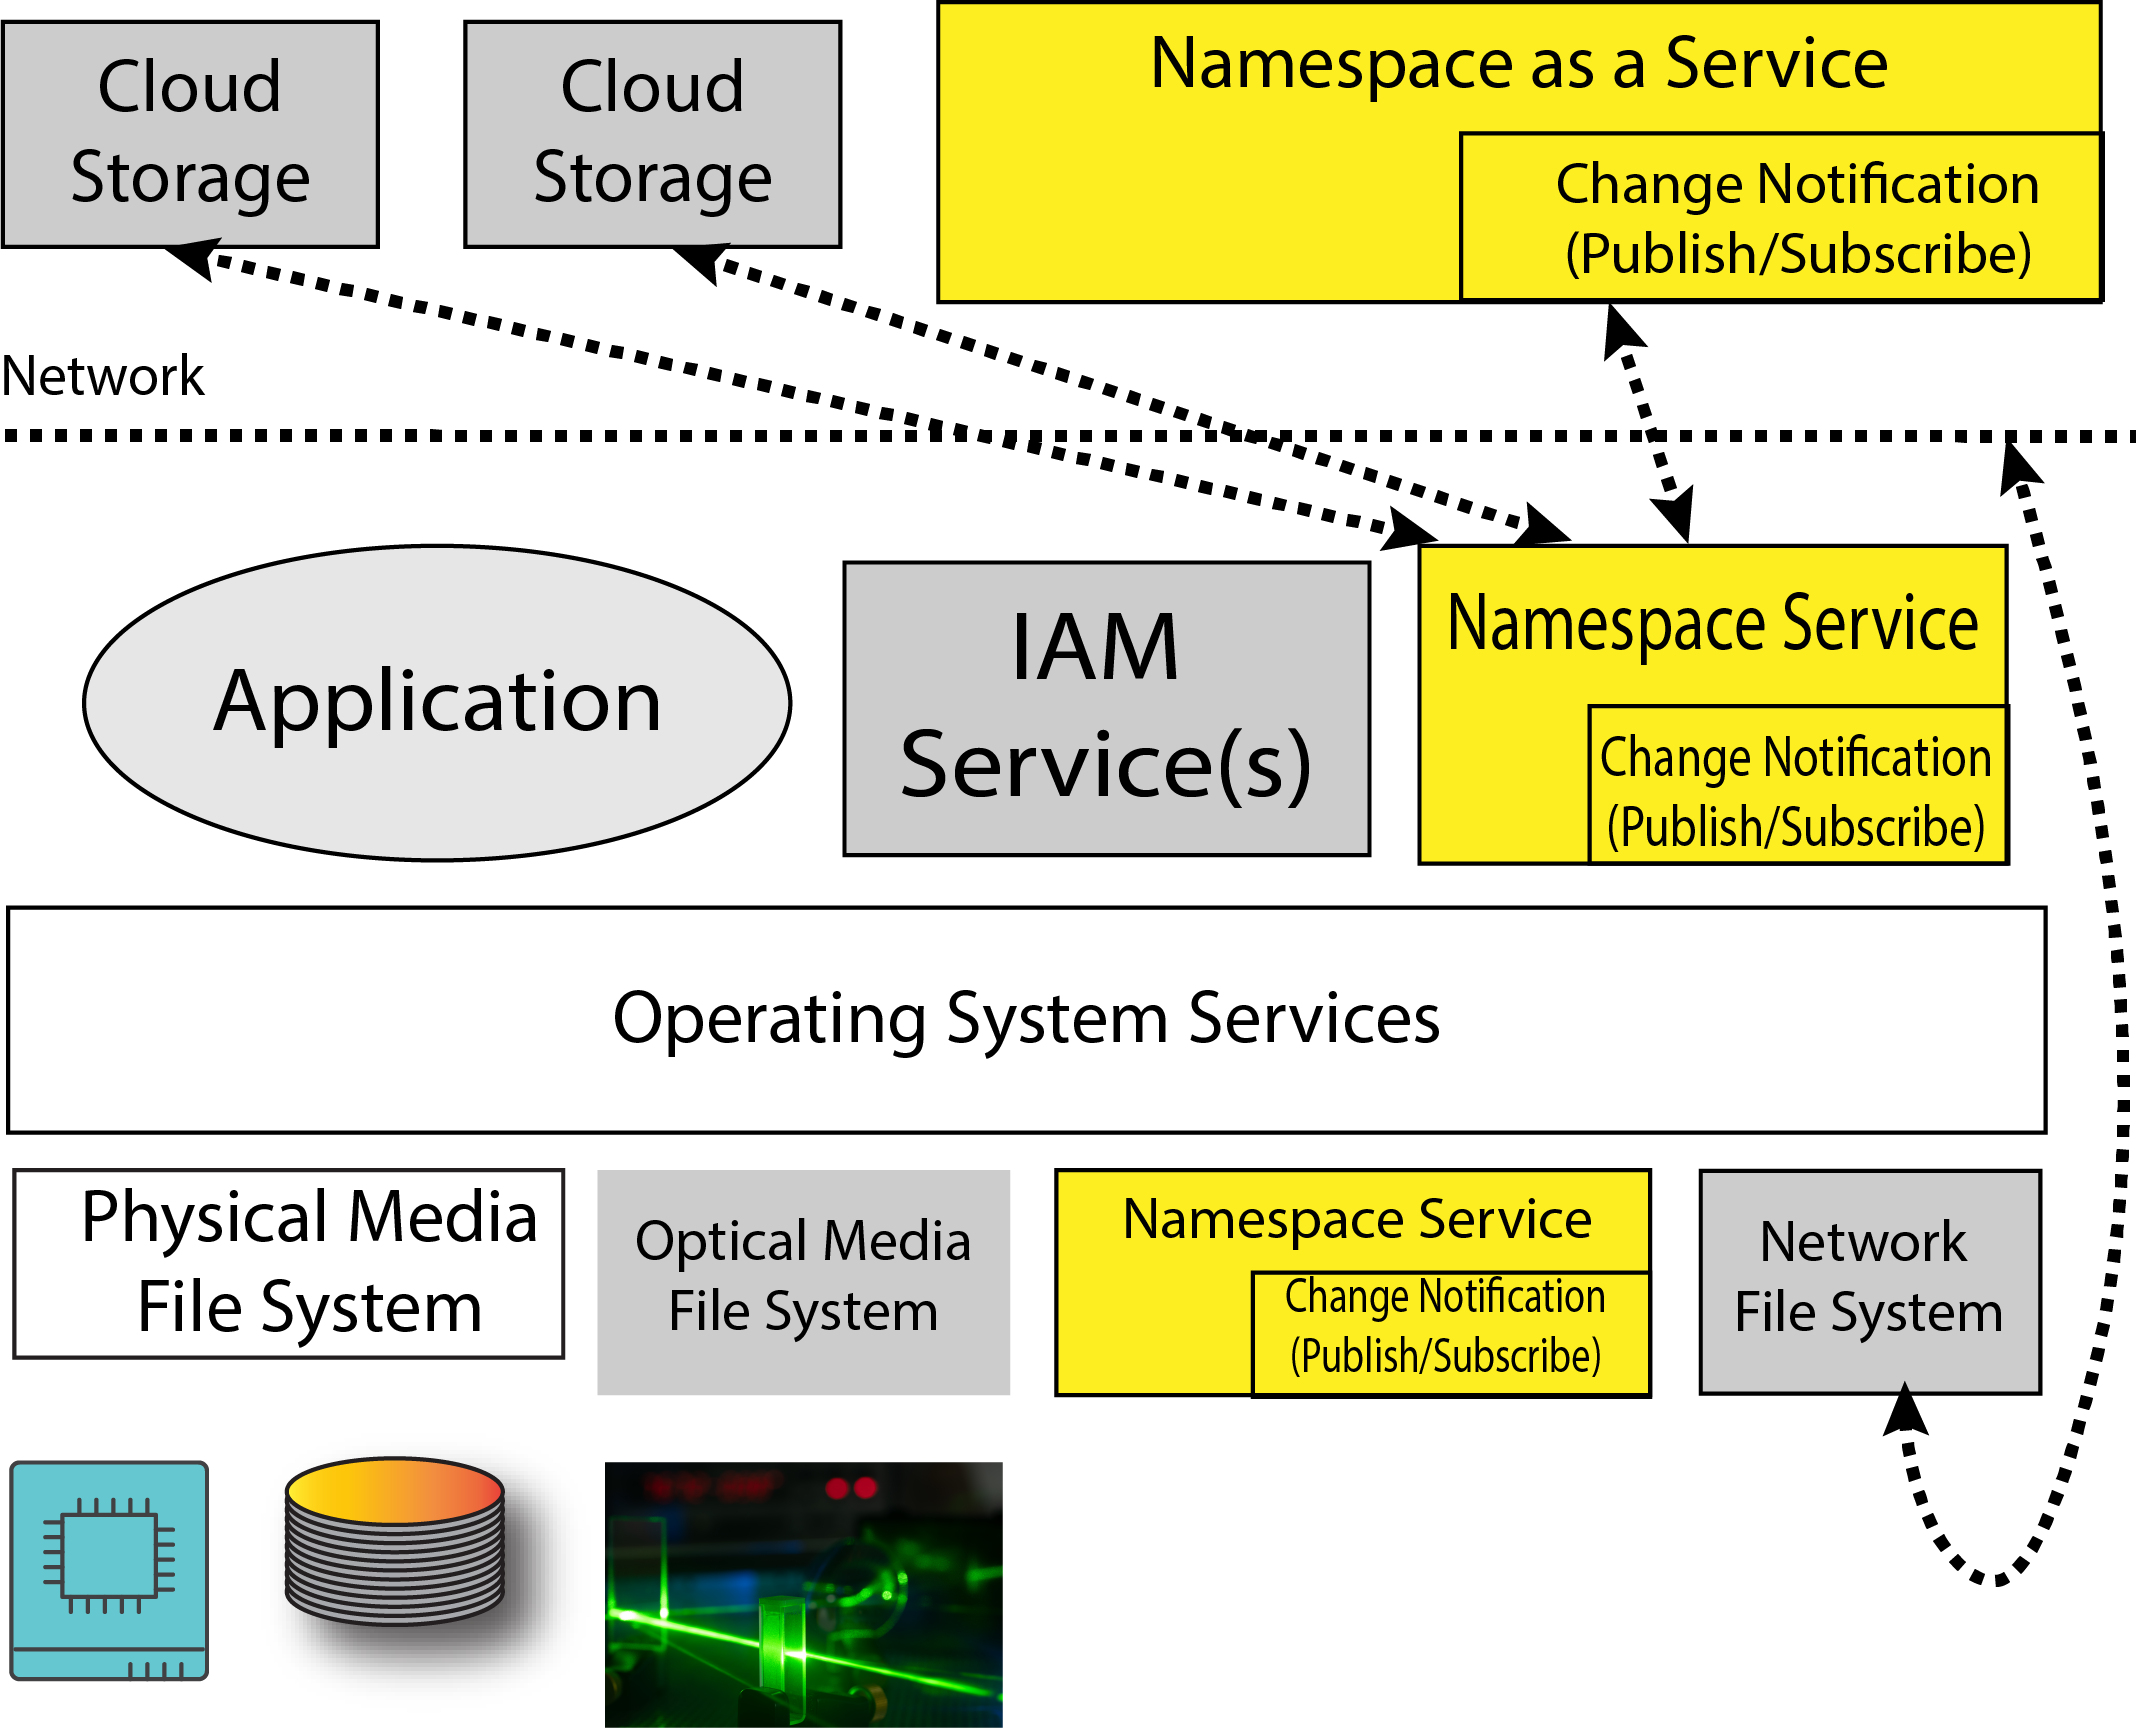
\includegraphics[width=0.95\columnwidth]{figures/nirvana-arch-8.png}
    \end{tabular}
    \caption{Nirvana Systems Architecture.}  %Separate Namespace service(s) from storage service(s).  Kernel namespace service permits use throughout OS lifetime, including boot.  User namespace service permits integration with remote namespace service and local namespace service, providing integration over the network.  Namespace as a Service (Naas) provides the ability to maintain shared namespaces across computational device boundaries; can provide primary or secondary name services.}
    \label{fig:systemsarchitecture}
\end{figure}

